\clearpage
\section*{Question 1}
\addcontentsline{toc}{section}{Question 1}

\begin{figure}[h!]
    \centering
    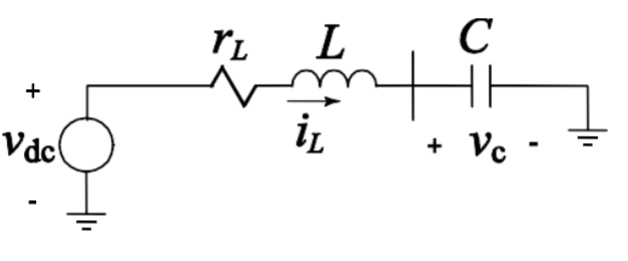
\includegraphics[width=0.8\textwidth]{figures/hw01_q01_circuit-diagram-a.png}
    \caption{Circuit diagram for a simple filter for questions 1-8}
    \label{fig:q01_circuit}
\end{figure}

A shunt harmonic filter (series $RLC$) is shown in \Cref{fig:q01_circuit} above. It is designed for a three-phase 13.8~kV 60~Hz system to shunt the 7th harmonic current. Find the reactive power, damped and undamped resonance frequency, and quality factor of the filter. The circuit parameters are: $r_L = 1~\Omega$, $L = 19~\text{mH}$, and $C = 8.2~\mu\text{F}$.

\vspace{1em}

\textbf{Step 1: Write the KVL equation:}
\begin{align*}
	V_{\rm dc} - r_L i_L - L \frac{di_L}{dt} - v_C = 0
\end{align*}
	\qquad Or equivalently:
\begin{align*}
	L \frac{d i_L}{dt} + r_L i_L + v_C = V_{\rm dc}
\end{align*}


\qquad With $i_L = C \frac{dv_C}{dt}$ and $v_C = \frac{1}{C} \int i_L dt$.
\vspace{1em}


\textbf{Step 2: Standard second-order ODE:}
\begin{align*}
	\frac{d^2 i_L}{dt^2} + \frac{r_L}{L} \frac{d i_L}{dt} + \frac{1}{LC} i_L = 0
\end{align*}

\textbf{Step 3: Characteristic equation:}
\begin{align*}
	s^2 + 2\zeta \omega_n s + \omega_n^2 = 0
\end{align*}

\textbf{Step 4: Calculate parameters:}
\begin{align*}
	\omega_n &= \frac{1}{\sqrt{LC}} = \frac{1}{\sqrt{19 \times 10^{-3} \times 8.2 \times 10^{-6}}} = 2533.5~\text{rad/s} \\
	\zeta &= \frac{r_L}{2 \sqrt{\frac{L}{C}}} = \frac{1}{2 \sqrt{\frac{19 \times 10^{-3}}{8.2 \times 10^{-6}}}} = 0.0104 \\
	\omega_d &= \omega_n \sqrt{1-\zeta^2} = 2533.3~\text{rad/s}
\end{align*}

\textbf{Quality factor:}
\begin{align*}
	Q_{\text{factor}} = \frac{\omega_n L}{r_L} = \frac{2533.5 \times 0.019}{1} = 48.136
\end{align*}

\textbf{Eigenvalues (roots of characteristic equation):}
\begin{align*}
	\lambda = -\zeta \omega_n \pm j \omega_d = -26.316 \pm 2533.3j
\end{align*}

\textbf{Reactive Power Computation:}
The reactive power is computed for a three-phase system. First, the per-phase voltage $V_{ph} = V_{LL}/\sqrt{3}$ and current $I_{ph}$ are calculated using the per-phase impedance $Z_{ph}=r_L + j(X_L - X_c)$. Then, the reactive power is determined as:
\begin{align*}
    Q_{\text{kVAr}} = 3 \times |I_{ph}|^2 \times X_c
\end{align*}
where $X_c = \frac{1}{2 \pi f C}$ and $X_L = 2 \pi f L$ at $f = 60~\text{Hz}$.


\begin{align*}
	Q_{\text{kVAr}} = -602.04~\text{kVAr}
\end{align*}

Negative sign indicates the filter is absorbing reactive power (capacitive).

All calculations confirm the system is very underdamped ($\zeta = 0.0104$).

\vspace{1em}
	\textbf{Summary of Key Results:}
\begin{itemize}
	\item Natural frequency: $\boxed{\omega_n = 2533.5~\text{rad/s}}$
	\item Damping ratio: $\boxed{\zeta = 0.0104}$
	\item Damped frequency: $\boxed{\omega_d = 2533.3~\text{rad/s}}$
	\item Quality factor: $\boxed{Q = 48.136}$
	\item Eigenvalues: $\boxed{-26.316 \pm 2533.3j}$
	\item Reactive power: $\boxed{-602.04~\text{kVAr}}$
\end{itemize}


